\chapter{Resultados}\label{chapter:resultados}

En el repositorio del proyecto \cite{padel-project} se pueden encontrar vídeos que muestran el comportamiento de los agentes entrenados, además de los resultados y modelos obtenidos tras el entrenamiento.

\section{Aprendizaje por refuerzo profundo}

El objetivo de la experimentación utilizando técnicas de aprendizaje por refuerzo profundo ha sido, principalmente, demostrar empíricamente que el entrenamiento de agentes virtuales en el entorno virtual de pádel es factible.

Otros aspectos que se han estudiado son el efecto que tiene utilizar Curiosity en este entorno, además de cómo afectan al entrenamiento la modificación de la función de recompensa, definida inicialmente en la prueba inicial.

En realidad, hay otros parámetros que se deberían haber estudiado durante la experimentación. Por ejemplo, hubiera sido relevante haber hecho más pruebas modificando los hiperparámetros de las redes neuronales utilizadas. Sin embargo, esto hubiera extendido demasiado la parte de experimentación, por lo que se optó por dar prioridad a experimentar con los elementos definidos directamente en el entorno virtual.

A la hora de comparar experimentos, las medidas que se han utilizado son las relacionadas con el entorno y la puntuación Elo:
\begin{enumerate}
    \item[-] Dentro de las recompensas del entorno están la recompensa acumulada y la duración de un episodio, y son relevantes para determinar si la política que se está entrenando correctamente. Normalmente, al principio del entrenamiento los episodios suelen ser cortos y la recompensa acumulada es usualmente muy variada, ya que la política aún no sabe mucho del entorno. A medida que va aprendiendo, la idea sería que la duración de los episodios y la recompensa acumulada de cada episodio aumentaran cada vez más. Específicamente en este entorno virtual de pádel, sin embargo, un aumento en la duración del episodio no necesariamente implicaría una mejora en la política. Por ejemplo, los agentes podrían aprender a mantener la pelota en juego realizando siempre golpeos muy fáciles de devolver, lo cual no es deseado.
    \item[-]  La puntuación Elo de la política resulta ser una medida más fiable que el resto, al tratarse de un entorno competitivo. Esta puntuación aumenta o decrementa en función de cómo está rindiendo la política que está siendo entrenada contra las instancias de políticas obtenidas con \emph{self-play}. La variación de la puntuación siempre depende del oponente, si por ejemplo se ganara a un oponente con una puntuación Elo mucho más alta, el propio agente ganaría más puntos. En cambio, si la puntuación del oponente fuera baja, ganaría muy pocos puntos. Si la puntuación Elo aumenta considerablemente durante el trascurso del entrenamiento, significaría que el agente está consiguiendo ganar a oponentes más hábiles que el propio agente.
\end{enumerate}

Aunque estas medidas ya aportan mucha información sobre cómo ha ido el entrenamiento, para saber si realmente se ha podido conseguir un modelo robusto, también es importante probar el modelo directamente a través de Unity, mediante inferencia, para comprobar si realmente ha podido aprender a jugar a pádel.

\newpage

\subsection{Experimento 1. Entrenamiento mediante PPO}

El primer experimento ha consistido en hacer una prueba sencilla en la que solo se definen recompensas por ganar y perder puntos, mostradas en la Tabla \ref{tab:exp1-rewards}. Para el entrenamiento se ha utilizado PPO, y la configuración del entrenamiento se puede consultar en el Apéndice \ref{appendix:config-file-ppo}.

\begin{table}[H]
\centering
    \begin{tabular}{|>{\rowmac}p{6.5cm}|>{\rowmac}c<{\clearrow}|} 
        \hline
        \multicolumn{1}{|c|}{\textbf{Recompensa}} & \multicolumn{1}{c|}{\textbf{Valor}} \\ \hline \hline
        \texttt{WinningReward} & $10$ \\
        \hline
        \texttt{LosingReward} & $-10$ \\
        \hline
        \texttt{ApproachingKeyPositionsReward} & $0$ \\
        \hline
        \texttt{StayingAroundKeyPositionsReward} & $0$ \\
        \hline
        \texttt{HittingBallReward} & $0$ \\
        \hline
    \end{tabular}
    \caption[Función de recompensa del experimento 1]{Función de recompensa del experimento 1. (Elaboración propia)}
    \label{tab:exp1-rewards}
\end{table}

Tras un millón de pasos, las medidas obtenidas han sido las mostradas en la Figura \ref{fig:exp1-plots}. Como es notable, la recompensa acumulada no ha dejado de variar hasta las últimas iteraciones del entrenamiento, en los que parece que uno de los dos equipos es capaz de ganar varios puntos seguidos. Eso se debe a que, al principio del entrenamiento, como que los agentes apenas han tenido tiempo para aprender nada, y al haber rotaciones en el servicio de la pelota, la obtención de puntos se va alternando constantemente. A medida que aumenta la duración de los episodios, cada juego se va volviendo más reñido, hecho que contribuye mucho en el proceso de aprendizaje. En cuanto a la puntuación Elo, se puede observar que ha ido subiendo a medida que avanzaba el entrenamiento, y parece que la política aún tenía margen de mejora, ya que en los últimos episodios el aumento seguía siendo bastante considerable.
\begin{figure} [H]
 \centering
  \subfloat[Recompensa acumulada]{
    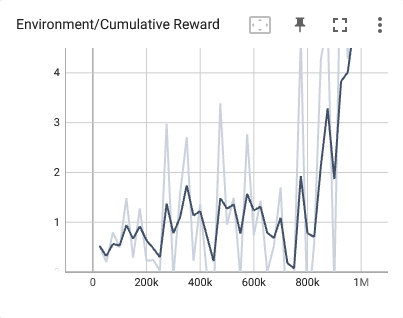
\includegraphics[width=0.325\textwidth]{figures/exp1-reward.png}}
  \subfloat[Duración del episodio]{
    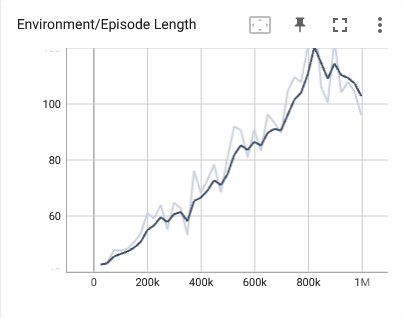
\includegraphics[width=0.325\textwidth]{figures/exp1-episode.png}}
  \subfloat[Puntuación Elo]{
    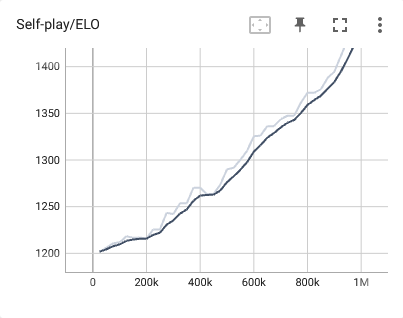
\includegraphics[width=0.325\textwidth]{figures/exp1-elo.png}}
 \caption[Resultados del experimento 1]{Resultados del experimento 1. (Elaboración propia)}
 \label{fig:exp1-plots}
\end{figure}

Finalmente, probando el modelo obtenido directamente en el entorno de Unity, se ha observado que en esta primera prueba el posicionamiento no era muy bueno. Durante el partido, los agentes acababan juntándose frecuentemente para ir hacia la pelota a la vez. En realidad, este comportamiento era el esperado, ya que las únicas recompensas que se habían definido fueron las obtenidas tras un punto, por los que los agentes no reciben ningún feedback sobre cómo se deberían posicionar. Otro aspecto destacable es que la política parece ser capaz de enviar la pelota hacia espacios libres, lo cual se podría considerar como un comportamiento muy competitivo, lo cual es bueno. Por ejemplo, en varias ocasiones, los agentes envían la pelota hacia el fondo cuando los oponentes se encuentran cerca de la red, dificultando el alcance de la pelota a los oponentes.

\subsection{Experimento 2. Efecto de Curiosity en el entorno virtual de pádel}

En este experimento se ha puesto a prueba el efecto que tendría añadir la recompensa intrínseca Curiosity a este entorno. Para hacer una comparación justa con los resultados obtenidos en el experimento anterior, se han definido las mismas recompensas extrínsecas. En cuanto a la configuración del entrenamiento, la cual se puede consultar en el Apéndice \ref{appendix:config-file-curiosity}, todos los parámetros se han mantenido igual salvo la adición de la configuración específica de Curiosity.

\begin{table}[H]
\centering
    \begin{tabular}{|>{\rowmac}p{6.5cm}|>{\rowmac}c<{\clearrow}|} 
        \hline
        \multicolumn{1}{|c|}{\textbf{Recompensa}} & \multicolumn{1}{c|}{\textbf{Valor}} \\ \hline \hline
        \texttt{WinningReward} & $10$ \\
        \hline
        \texttt{LosingReward} & $-10$ \\
        \hline
        \texttt{ApproachingKeyPositionsReward} & $0$ \\
        \hline
        \texttt{StayingAroundKeyPositionsReward} & $0$ \\
        \hline
        \texttt{HittingBallReward} & $0$ \\
        \hline
    \end{tabular}
    \caption[Función de recompensa del experimento 2]{Función de recompensa del experimento 2. (Elaboración propia)}
    \label{tab:exp2-rewards}
\end{table}
Las medidas obtenidas en este experimento (y en los experimentos de ahora en adelante) se han contrastado con los resultados obtenidos en el experimento sin Curiosity (de color azul marino para todas las gráficas). Observando la Figura \ref{fig:exp2-plots}, resulta evidente que el uso de Curiosity no solo no ha aportado ninguna mejora, sino que además ha empeorado el rendimiento de los agentes. La recompensa acumulada ha tenido mucha varianza durante todo el entrenamiento, y la duración de los episodios no ha aumentado mucho. La puntuación Elo empeoraba cada vez más durante la primera mitad del entrenamiento, y después se la primera mitad prácticamente se mantuvo constante.

La conclusión sacada tras estas pruebas es que parece que condicionar a los agentes incentivándoles a explorar nuevos estados no es muy adecuado en este tipo de entornos de aprendizaje. Esto se debe muy posiblemente a que se trata de un entorno cerrado, en el que el objetivo es muy claro: dirigirse hacia la pelota y devolverla al campo contrario. Con Curiosity, los agentes son recompensados aunque se estén alejando de la pelota, y necesitarían muchísimos más pasos de entrenamiento hasta que aprendan cuál es exactamente el objetivo que tienen, una vez el peso de las recompensas intrínsecas Curiosity sea prácticamente nulo.

\begin{figure} [H]
 \centering
  \subfloat[Recompensa acumulada]{
    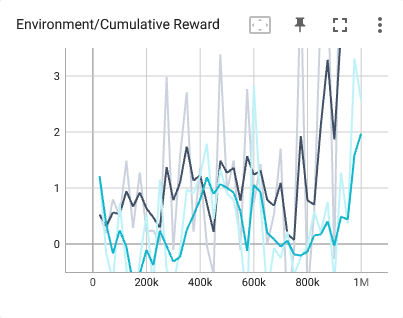
\includegraphics[width=0.325\textwidth]{figures/exp2-reward.png}}
  \subfloat[Duración del episodio]{
    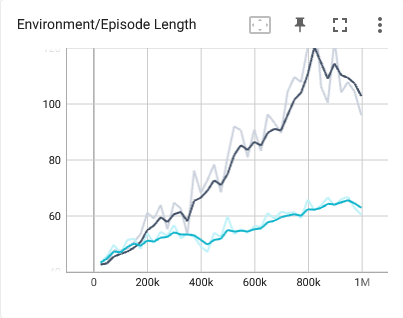
\includegraphics[width=0.325\textwidth]{figures/exp2-episode.png}}
  \subfloat[Puntuación Elo]{
    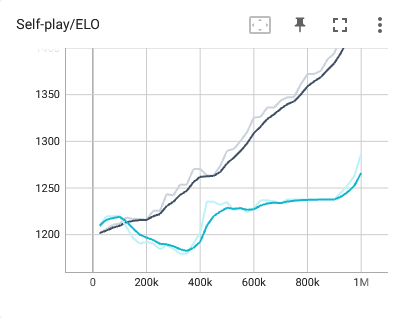
\includegraphics[width=0.325\textwidth]{figures/exp2-elo.png}}
 \caption[Resultados del experimento 2]{Resultados del experimento 2, en azul. (Elaboración propia)}
 \label{fig:exp2-plots}
\end{figure}

Desde el entorno de Unity, enfrentando el modelo sin Curiosity contra el modelo obtenido en este experimento, se puede observar que los agentes entrenados con Curiosity la mayoría de veces ni siquiera son capaces de dirigirse a la pelota.

\subsection{Experimento 3. Influencia de la recompensa por golpeo}

En el entorno de pádel, una manera de evitar la escasez de recompensas es añadiendo una recompensa por golpear la pelota. Con esta recompensa, los agentes deberían poder aprender más rápidamente que uno de los objetivos que tienen es devolver la pelota hacia el campo rival. En el tercer experimento, se ha utilizado esta recompensa para determinar si realmente influye en el entrenamiento de los agentes. Tanto en este como en los experimentos restantes se han utilizado la configuración del entrenamiento utilizada en el primer experimento, ya que Curiosity no ha resultado ser efectivo.

\begin{table}[H]
\centering
    \begin{tabular}{|>{\rowmac}p{6.5cm}|>{\rowmac}c<{\clearrow}|} 
        \hline
        \multicolumn{1}{|c|}{\textbf{Recompensa}} & \multicolumn{1}{c|}{\textbf{Valor}} \\ \hline \hline
        \texttt{WinningReward} & $10$ \\
        \hline
        \texttt{LosingReward} & $-10$ \\
        \hline
        \texttt{ApproachingKeyPositionsReward} & $0$ \\
        \hline
        \texttt{StayingAroundKeyPositionsReward} & $0$ \\
        \hline
        \texttt{HittingBallReward} & $1$ \\
        \hline
    \end{tabular}
    \caption[Función de recompensa del experimento 3]{Función de recompensa del experimento 3. (Elaboración propia)}
    \label{tab:exp3-rewards}
\end{table}

En los resultados de este experimento, el cambio más notable ha sido en la recompensa acumulada. Al haber una recompensa por golpear la pelota, en general, los agentes acaban obteniendo más recompensas en cada episodio, por lo que este variación era de esperarse. La diferencia entre la duración de los episodios no es tan clara, ya que aunque durante la mitad del entrenamiento la duración estuviera por debajo del primer experimento, al final del entrenamiento se acabó superando. En la puntuación Elo también pasa algo similar, parece que la política de este experimento tiende a mejorar más rápidamente, pero al final del entrenamiento apenas aumenta. En principio, parece que la recompensa por golpear la pelota no ha sido de gran utilidad. Quizás se debe mayoritariamente a que, dentro de lo que cabe, las recompensas que se dan tras cada punto no están tan alejadas entre sí.

Como apunte, es importante tener en consideración que las recompensas deben definirse en proporción a lo relevantes que sean respecto al objetivo final. En este caso, por ejemplo, la recompensa que se ha definido por golpear la pelota es, quizás, demasiado alta en comparación a la recompensa por ganar un punto: tras diez golpeos en un punto, la recompensa por ganar ese punto acaba perdiendo relevancia. Esto puede conllevar a que los agentes adopten comportamientos que les permita explotar estas recompensas más pequeñas, haciendo que ambos equipos cooperen para sumar puntos en lugar de ser competitivos.

\begin{figure} [H]
 \centering
  \subfloat[Recompensa acumulada]{
    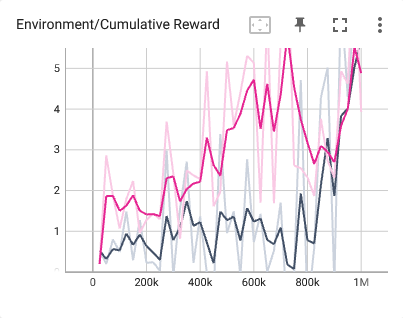
\includegraphics[width=0.325\textwidth]{figures/exp3-reward.png}}
  \subfloat[Duración del episodio]{
    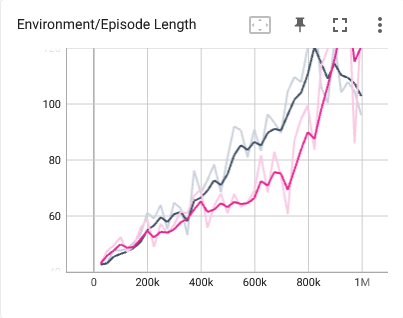
\includegraphics[width=0.325\textwidth]{figures/exp3-episode.png}}
  \subfloat[Puntuación Elo]{
    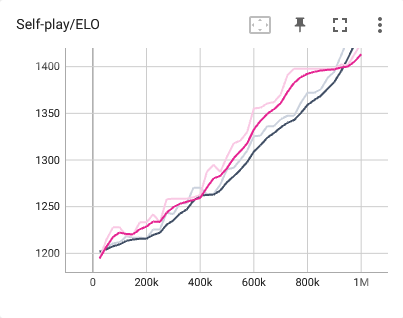
\includegraphics[width=0.325\textwidth]{figures/exp3-elo.png}}
 \caption[Resultados del experimento 3]{Resultados del experimento 3, en magenta. (Elaboración propia)}
  \label{fig:exp3-plots}
\end{figure}

\subsection{Experimento 4. Importancia del sistema de puntuación Elo}

Derivado del tercer experimento, en el cuarto experimento se ha forzado el problema de la explotación eliminando la recompensa por ganar un punto. Nótese que aunque esta recompensa pase a ser cero, sería equivalente si la recompensa por golpear la pelota fuera excesivamente grande.

\begin{table}[H]
\centering
    \begin{tabular}{|>{\rowmac}p{6.5cm}|>{\rowmac}c<{\clearrow}|} 
        \hline
        \multicolumn{1}{|c|}{\textbf{Recompensa}} & \multicolumn{1}{c|}{\textbf{Valor}} \\ \hline \hline
        \texttt{WinningReward} & $0$ \\
        \hline
        \texttt{LosingReward} & $-10$ \\
        \hline
        \texttt{ApproachingKeyPositionsReward} & $0$ \\
        \hline
        \texttt{StayingAroundKeyPositionsReward} & $0$ \\
        \hline
        \texttt{HittingBallReward} & $1$ \\
        \hline
    \end{tabular}
    \caption[Función de recompensa del experimento 4]{Función de recompensa del experimento 4. (Elaboración propia)}
    \label{tab:exp4-rewards}
\end{table}

Tal y como se esperaba, en los resultados de este experimento se puede observar cómo tanto la recompensa acumulada como la duración de un episodio han aumentado drásticamente, a partir de la segunda mitad del entrenamiento. Al principio, las recompensas acumuladas son negativas debido a que los agentes aún no son capaces de golpear la pelota. A medida que van aprendiendo, ambos equipos acaban descubriendo que son capaces de prácticamente anular la penalización por perder un punto, si cooperan entre sí para devolverse la pelota constantemente. La duración de un episodio aumenta precisamente por esta razón.

Sin embargo, cabe destacar que la variación en la puntuación Elo ha sido justo lo contrario. Aunque a primera vista parecía que los agentes habían aprendido una buena política, la puntuación Elo indica que apenas están mejorando. Esto se debe precisamente a que, al final de cada episodio, realmente no hay ningún equipo que pierda, ya que la recompensa acumulada de ambos equipos acaba siendo positiva. Es precisamente por este motivo que el sistema de puntuación Elo es, a veces, más relevante que las otras medidas, ya que ofrece una mejor valoración del rendimiento en los entornos competitivos.

\begin{figure} [H]
 \centering
  \subfloat[Recompensa acumulada]{
    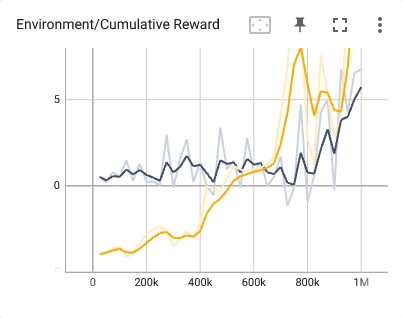
\includegraphics[width=0.325\textwidth]{figures/exp4-reward.png}}
  \subfloat[Duración del episodio]{
    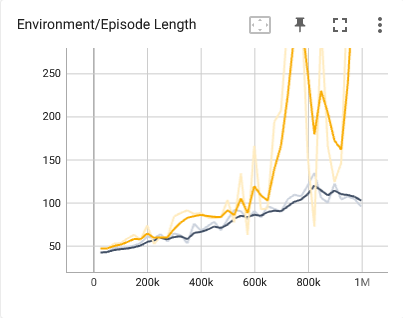
\includegraphics[width=0.325\textwidth]{figures/exp4-episode.png}}
  \subfloat[Puntuación Elo]{
    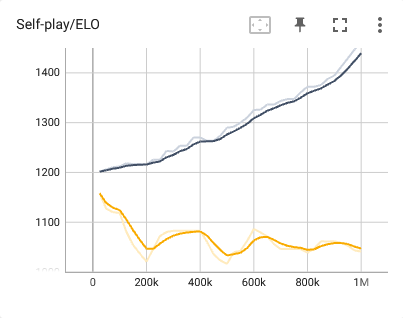
\includegraphics[width=0.325\textwidth]{figures/exp4-elo.png}}
 \caption[Resultados del experimento 4]{Resultados del experimento 4, en amarillo. (Elaboración propia)}
  \label{fig:exp4-plots}
\end{figure}

Infiriendo el modelo obtenido en los agentes desde Unity, se puede observar que la mayoría de golpeos que realizan son globos. Esto es así porque los agentes ya saben que se trata de la opción más segura para garantizar una devolución constante entre ambos equipos. También cabe mencionar que, pese a que no son agentes muy ofensivos, cuando se trata de dirigirse hacia la pelota y devolverla, actúan bastante bien.

\subsection{Experimento 5. Influencia de las posiciones clave}

Para el último experimento se ha analizado el efecto que tienen las recompensas asociadas a los puntos clave. Como son recompensas que se pueden conseguir de manera continua durante un episodio, estas deben ser lo suficientemente pequeñas como para no sobrepasar las recompensas principales.

\begin{table}[H]
\centering
    \begin{tabular}{|>{\rowmac}p{6.5cm}|>{\rowmac}c<{\clearrow}|} 
        \hline
        \multicolumn{1}{|c|}{\textbf{Recompensa}} & \multicolumn{1}{c|}{\textbf{Valor}} \\ \hline \hline
        \texttt{WinningReward} & $10$ \\
        \hline
        \texttt{LosingReward} & $-10$ \\
        \hline
        \texttt{ApproachingKeyPositionsReward} & $0\text{.}005$ \\
        \hline
        \texttt{StayingAroundKeyPositionsReward} & $0\text{.}01$ \\
        \hline
        \texttt{HittingBallReward} & $0$ \\
        \hline
    \end{tabular}
    \caption[Función de recompensa del experimento 5]{Función de recompensa del experimento 5. (Elaboración propia)}
    \label{tab:exp5-rewards}
\end{table}

En los resultados del experimento 5, se puede apreciar una ligera mejora en el rendimiento de los agentes, justamente al final del entrenamiento. Aun así, esta mejora no es tan distinguida como se esperaba.

Mediante las posiciones clave, la idea era que los agentes pudieran ser capaces de aprender mucho antes dónde se deberían posicionar. Es probable que esto no haya sido posible debido a factores como:
\begin{enumerate}
    \item[-] La magnitud de las recompensas, ya que al ser tan pequeñas, los agentes no le dan demasiada relevancia.
    \item[-] Falta de coherencia con las observaciones, ya que los agentes, aunque ganen estas recompensas, difícilmente las pueden asociar con las posiciones de interés, ya que no disponen información de estas.
    \item[-] Las circunstancias en las que se obtienen, porque las posiciones de interés quizás son demasiado específicas, y habría que probar a hacer cambios para generalizarlo. Por ejemplo, escalar la recompensa por acercarse a una recompensa, según cuánto se haya acercado realmente dentro de un intervalo de tiempo, penalizar si un agente está demasiado tiempo en una posición poco deseada, etc.
\end{enumerate}
Aunque el uso de las posiciones de interés no haya sido muy efectiva en esta versión, su implementación sirve como base para definir funciones de recompensas más complejas.

\begin{figure} [H]
 \centering
  \subfloat[Recompensa acumulada]{
    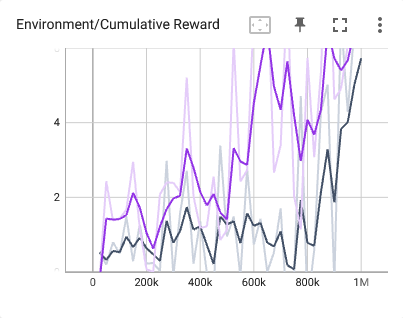
\includegraphics[width=0.325\textwidth]{figures/exp5-reward.png}}
  \subfloat[Duración del episodio]{
    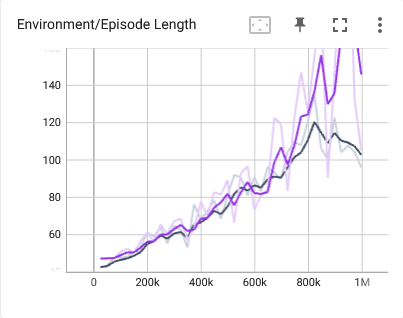
\includegraphics[width=0.325\textwidth]{figures/exp5-episode.png}}
  \subfloat[Puntuación Elo]{
    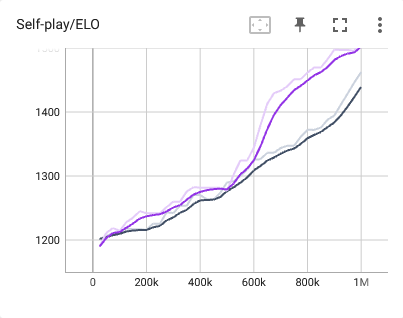
\includegraphics[width=0.325\textwidth]{figures/exp5-elo.png}}
 \caption[Resultados del experimento 5]{Resultados del experimento 5, en morado. (Elaboración propia)}
  \label{fig:exp5-plots}
\end{figure}

\newpage

\section{Aprendizaje por imitación}

La experimentación con el aprendizaje por imitación ha revelado una serie de obstáculos que limitan considerablemente el aprendizaje de los agentes. Dichos obstáculos están relacionados con las dificultades surgidas durante la grabación de demostraciones.

El principal problema es la latencia resultante de la decisión de establecer una conexión cliente-servidor para el intercambio de datos.

Aunque el envío de solicitudes se haya implementado de manera eficiente, esto no sirve de mucho cuando es la propia conexión la que introduce un tiempo de espera. Teniendo en cuenta que el entorno se va ejecutando contínuamente, donde el intervalo de tiempo entre un fotograma y otro es mínimo, resulta inviable que los agentes puedan moverse únicamente cada 0.2 segundos, por ejemplo.

Solucionar el problema de la latencia hubiera implicado rediseñar la manera en la que se obtienen los datos. Por ejemplo, se podría haber considerado implementar los árboles decisionales directamente en el entorno de Unity, aunque esto podría causar problemas de rendimiento, afectando a la tasa de fotogramas. Sin embargo, esto no ha sido posible debido a las limitaciones de tiempo.

Aun así, observando cómo se comportaban los agentes guiados por el entrenador, fueron notables algunos problemas que se deberían tener en cuenta de cara a una futura implementación:
\begin{enumerate}
    \item[-] El conjunto de datos, al ser muy escaso teniendo en cuenta que la búsqueda se realiza en un espacio 10-dimensional, es muy probable que los agentes acaben realizando secuencias de acciones de manera cíclica (sobre todo cuando los estados iniciales están predefinidos, como es en el caso de este entorno). Una solución a esto sería, en vez de obtener únicamente la muestra más cercana, que se obtengan $n > 1$ muestras más cercanas, para escoger una acción entre estas.
    \item[-] Al haber coherencia temporal en los datos, muchas posiciones están muy próximas a otras. Esto hace que los agentes no puedan obtener demostraciones de muchos estados desconocidos, por lo que sería difícil generalizar la política del agente.
    \item[-] Es importante tener información sobre la velocidad de la pelota, ya que las decisiones son distintas según si la pelota va hacia un lado u otro, o cómo de rápido esté llegando. Este último aspecto sería fácil de incorporar, a partir de los datos de partidos reales, si únicamente se considera la velocidad 2D (ignorando la altura).
\end{enumerate}

Pese a estos problemas, ignorando el hecho de que los agentes realizaban acciones con demasiada lentitud, se podía apreciar que los movimientos eran menos erráticos, ya que en ocasiones eran capaces de acercarse a la pelota y devolverla. Esto ha servido para confirmar que el planteamiento ha sido correcto, por lo que en el futuro se planea entrenar los agentes durante mucho más tiempo y evaluar los resultados, tras optimizar el rendimiento del entrenador y la comunicación entre procesos.  